\section{Αμφιωτική Κρουστική Απόκριση Δωματίου - BRIR} \label{sec:BRIR}

Όταν ένας ήχος εκπέμπεται από μια πηγή σε έναν κλειστό χώρο, ένας ακροατής αρχικά θα λάβει τον άμεσο ήχο, ακολουθούμενο από ανακλάσεις από τους τοίχους ή αντικείμενα τοποθετημένα μέσα στο δωμάτιο, όπως φαίνεται στο Σχήμα \ref{fig:listener_reverberant_room}. 

\begin{figure}[h]
  \centering
  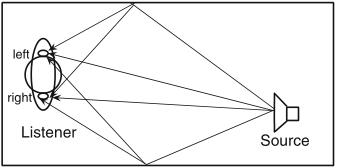
\includegraphics[width=\textwidth]{listener_reverberant_room.png}
  \caption{Ακροατής και ακουστική πηγή σε δωμάτιο με αντήχηση}
  \label{fig:listener_reverberant_room}
\end{figure}

Η ενέργεια του ανακλώμενου ήχου εξασθενεί, σύμφωνα με τα χαρακτηριστικά απορρόφησης των εκάστοτε επιφανειών στο δωμάτιο. Υποθέτοντας ότι η ακουστική του δωματίου, μοντελοποιείται ως ένα \textit{γραμμικό, χρονικά-αμετάβλητο} (ΓΧΑ), σύστημα, η κρουστική απόκριση του δωματίου, (Room Impulse Response - RIR), παρέχει μια πλήρη περιγραφή των άμεσων και ανακλώμενων μονοπατιών από μια πηγή στον δέκτη. Ο χρόνος που χρειάζεται για να ελαττωθεί η ενέργεια του δωματίου κατά 60 dB, αφού η πηγή έχει σταματήσει να εκπέμπει καλείται χρόνος αντήχησης $RT_{60}$ και είναι η παράμετρος που χρησιμοποιείται πιο συχνά για τον προσδιορισμό των ακουστικών ιδιοτήτων ενός δωματίου \cite{Tsilfidis2013}. Σε ένα γενικό, πολυκαναλικό σενάριο, με μία πηγή και \textit{i} δέκτες, το αντιχητικό σήμα $x_i(n)$, μπορεί να εκφραστεί σαν την συνέλιξη του ανηχοϊκού σήματος $s(n)$, με τις αντίστοιχες RIR, $h_i(n)$, ως εξής:

\begin{CEquation}
    x_i(n) = \sum_{j=0}^{J_h - 1} h_i(j)s(n-j) \label{eq 1}
\end{CEquation}

Όπου n αναπαριστά τον δείκτη διακριτού χρόνου και $J_h$ το μήκος της κρουστικής απόκρισης.

Σε ένα αμφιωτικό σενάριο (binaural) η απόκριση του δωματίου, συνδυάζεται με την κρουστική απόκριση του κεφαλιού (Head Related Impulse Response - HRIR), η οποία αποτελείται από δύο κανάλια, ένα για κάθε αυτί. Οι HRIR μετρούνται σε ανηχοϊκές συνθήκες. Συνεπώς, υποθέτοντας μια ιδεατή παντοκατευθυντική πηγή, μία αμφιωτική κρουστική απόκριση δωματίου, για το αριστερό αυτί-κανάλι, $h_L(n)$, μπορεί να εκφραστεί ως

\begin{CEquation}
\begin{split}
    h_L(n) = g(r_s)δ(n-n_s) * h_{\textit{HRIR},L,\theta_d,\phi_d}(n) \\+  \sum_{m=0}^{J_{h_m} - 1} h_{m,L}(n)*h_{\textit{HRIR},L,\theta_m,\phi_m}(n) \label{eq 2}
\end{split}
\end{CEquation}

όπου $g(r_s)$ είναι η ελάτωση του κέρδους που εξαρτάται από την απόσταση πηγής-παρατηρητή $r_s$, $\delta(n)$ η συνάρτηση δέλτα του Kronecker, $n_s$ η καθυστέρηση που εξαρτάται κυρίως από την απόσταση πηγής-παρατηρητή και τα φυσικά χαρακτηριστικά του μέσου διέλευσης. $h_{\textit{HRIR},L,\theta_m,\phi_m}(n)$ είναι η αριστερή HRIR για τον άμεσο ήχο, που αντιστοιχεί σε $\theta_d$ και $\phi_d$, δηλαδή την οριζόντια και κάθετη γωνία μεταξύ του παρατηρητή και της πηγής. Η τιμή $h_m(n)$ αναφέρεται στην m-οστή ανάκλαση. $J_{h_m}$ ο συνολικός αριθμός ανακλάσεων. Τέλος $\theta_m$ and $\phi_m$ είναι οι οριζόντιες και κάθετες γωνίες μεταξύ του δέκτη και της m-οστής ανάκλασης. Αντίστοιχα υπολογίζεται και η BRIR, $h_R(n)$. 

Έτσι, το αντηχητικό σήμα στο αριστερό και δεξί αυτί ενός ακροατή $x_L(n)$ και $x_R(n)$, περιγράφονται με τη συνέλιξη του ανηχοϊκού σήματος $s(n)$, με τις BRIR του αριστερού και δεξιού αυτιού αντίστοιχα, όπως φαίνεται στην Εξίσωση \ref{eq 3}.  Ένα παράδειγμα BRIR από ένα δωμάτιο με ιδιαίτερα υψηλή αντήχηση φαίνεται στο Σχήμα \ref{fig:BRIR_example}

\begin{CEquation}
\begin{split}
    x_L(n) = \sum_{j=0}^{J_{h_L} - 1} h_L(j)s(n-j) \\  \label{eq 3}
    x_R(n) = \sum_{j=0}^{J_{h_R} - 1} h_R(j)s(n-j)
\end{split}
\end{CEquation}

\begin{figure}[H]
  \centering
  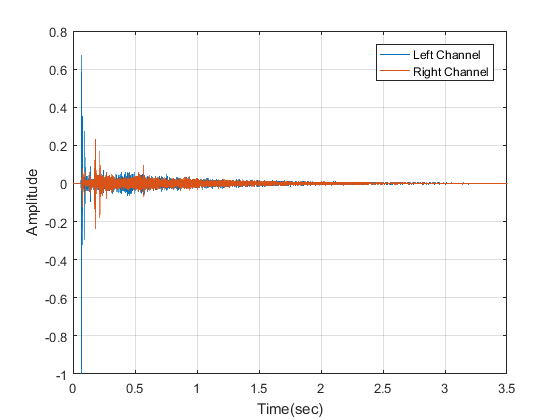
\includegraphics[width=\textwidth]{images/BRIR_example.png}
  \caption{BRIR από δωμάτιο με υψηλή αντίχηση}
  \label{fig:BRIR_example}
\end{figure}